\documentclass{article}
\usepackage{subfigure}
\usepackage[linesnumbered,ruled,vlined]{algorithm2e}
\usepackage{blindtext}
\usepackage{PRIMEarxiv}
\usepackage{amsmath,amssymb,amsthm} 
\usepackage{mathrsfs}
\usepackage[utf8]{inputenc} % allow utf-8 input
\usepackage[T1]{fontenc}    % use 8-bit T1 fonts
\usepackage{hyperref}       % hyperlinks
\usepackage{url}            % simple URL typesetting
\usepackage{booktabs}       % professional-quality tables
\usepackage{amsfonts}       % blackboard math symbols
\usepackage{nicefrac}       % compact symbols for 1/2, etc.
\usepackage{microtype}      % microtypography
\usepackage{lipsum}
\usepackage{graphicx}
\graphicspath{{Figures/}}     % organize your images and other figures under Figures/ folder
\usepackage{multicol}
\usepackage{algorithm}
\usepackage{algpseudocode}
\usepackage{amsmath}
\usepackage{caption}
\usepackage{subcaption}
\usepackage{geometry}
\setlength{\textfloatsep}{1pt}



%% Title
\title{STATS 403 Final Project Report: RSNA Screening Mammography Breast Cancer Detection}

\author{
\And
  Chenglin Zhang \\
  \texttt{cz155@duke.edu} \\
  %% examples of more authors
   \And
  Yijia Xue \\
  \texttt{yx179@duke.edu} \\
   \And
  Lihui Chen\\
  \texttt{@duke.edu} \\
}





\begin{document}
\maketitle
% keywords can be removed
\keywords{ }
\section*{Abstract}


\newpage
\tableofcontents
\newpage
\section{Problem Introduction}
\subsection{Background Information, Importance \& Motivation  }

\subsection{Difficulties of the problem}


\section{Literature Review}
\subsection{Medical Images Related Task Setting Taxonomy}
\subsection{Mammography Breast Cancer Detection}
\section{Project Research Contents}

\subsection{Dataset and Class Imbalance}

\subsection{Data Preprocess Techniques}

\subsection{Implenmented Model and Methodology}

\subsubsection{U-Net}
The typical use of convolutional networks is on classification tasks, where the output of an image is a single class label. However, in many visual tasks,
especially in biomedical image processing, the desired output should include localization, i.e., a class label is supposed to be assigned to each pixel. Moreover, thousands of training images are usually beyond reach in biomedical tasks.
\\\\
introduction
related work
explanation and quality of approach
explanation and quality of experiments / theoretical arguments and results
description of what each team member did

The U-Net is widely known for medical image segmentation.
\begin{figure}[htp]
    \centering
    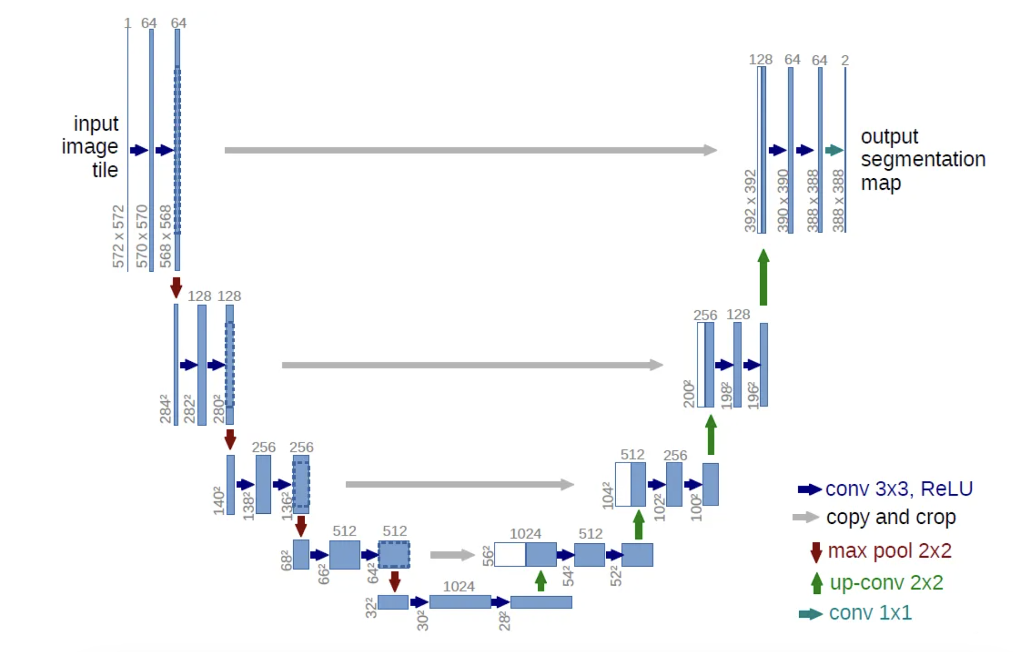
\includegraphics[scale = 0.8]{Figures/U-Net Architecture.png}
   \caption{Basic Structure of the U-Net}
\end{figure}
new line

Overlap-tile strategy for seamless segmentation of arbitrary large images. Prediction of the segmentation in the yellow area, requires image data within the blue area as input. Missing input data is extrapolated by mirroring. \\\\
Because the edge part is no more continuous after cutting (which made the final concatenation difficult). The overlap-tile strategy is adopted.
\paragraph{Skip-tile Strategy}
\begin{figure}[htp]
    \centering
    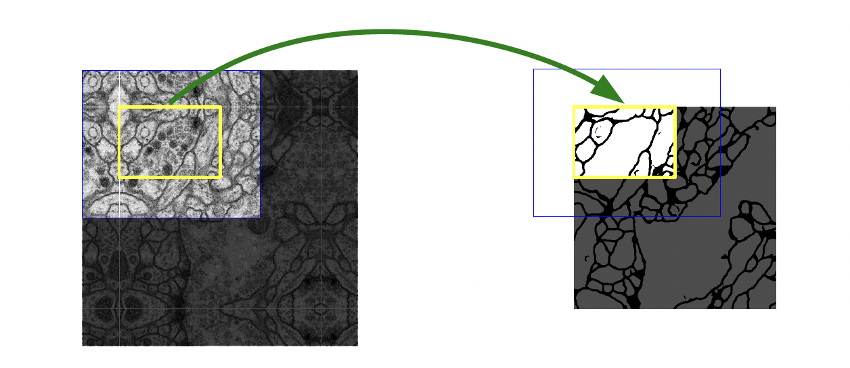
\includegraphics[scale = 0.5]{Figures/Skip-tile.png}
   \caption{Basic Structure of the U-Net}
\end{figure}

\paragraph{Image Interpolation}
\begin{align*}
    & X_{src} = (X_{dst} + 0.5) \times \frac{Width_{src}}{Width_{dst}} - 0.5 \\
    & Y_{src} = (Y_{dst} + 0.5) \times \frac{Height_{src}}{Height_{dst}} - 0.5 \\
\end{align*}
Bilinear Interpolation
\begin{figure}[htp]
    \centering
    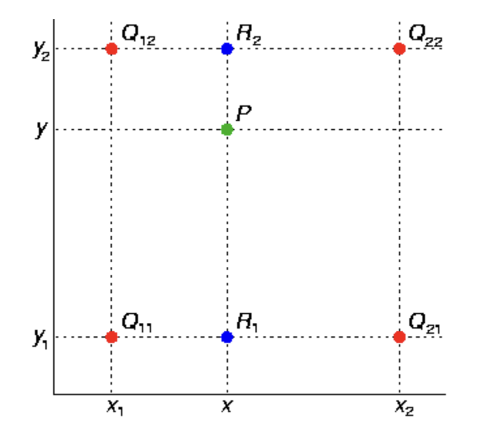
\includegraphics[scale = 0.5]{Figures/Bilinear Interpolation.png}
   \caption{Basic Structure of the U-Net}
\end{figure}

% \begin{figure}[htp]
%     \centering
%     \includegraphics[scale = 0.5]{Figures/.png}
%    \caption{Basic Structure of the U-Net}
% \end{figure}
\paragraph{Loss Function}
Firstly, the U-Net uses 
\begin{align*}
    p_k(x) = \exp{a_k(x)}/ \left(\sum_{K}{k'=1}\exp(a_{k'}(x))\right)
\end{align*}

\paragraph{The implications of the U-Net in our project}
\begin{figure}[htp]
    \centering
    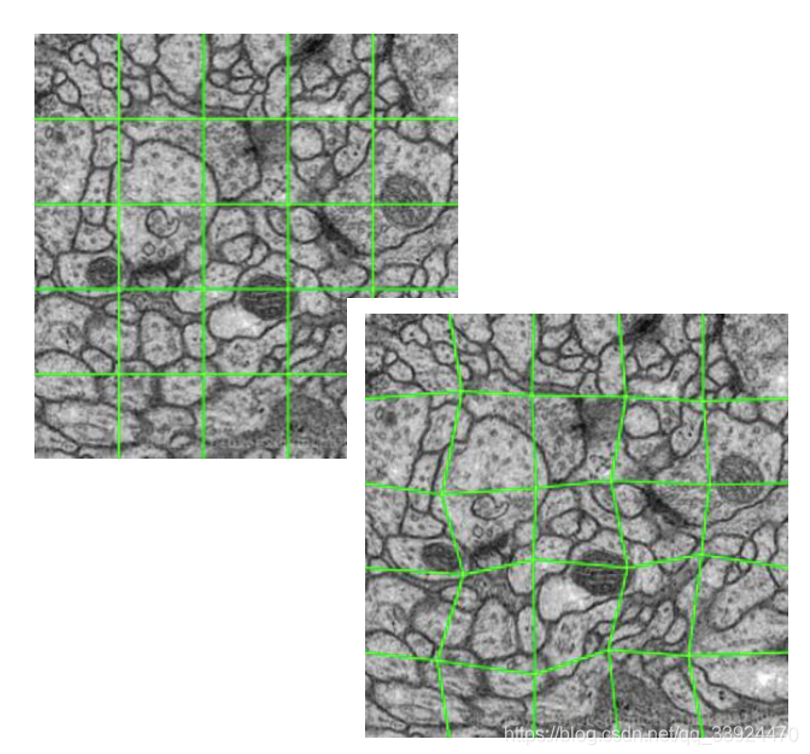
\includegraphics[scale = 0.5]{Figures/Distortion.png}
   \caption{Basic Structure of the U-Net}
\end{figure}
\subsubsection{Image Preprocessing}
\begin{figure}[htp]
    \centering
    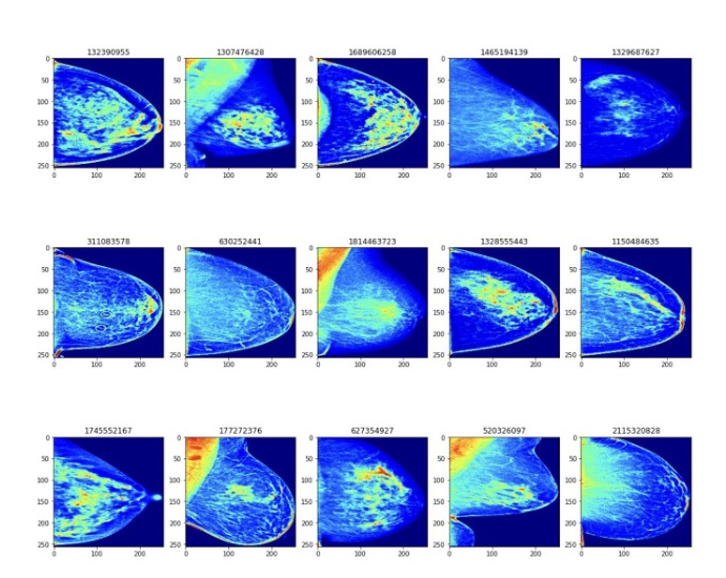
\includegraphics[scale = 0.8]{Figures/Pre-processed-data.png}
   \caption{Basic Structure of the U-Net}
\end{figure}
\begin{figure}[htp]
    \centering
    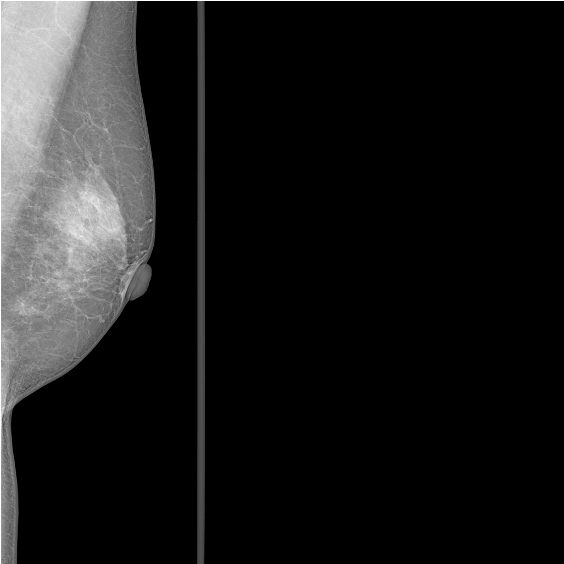
\includegraphics[scale = 0.5]{Figures/Bounding-Box.png}
   \caption{Basic Structure of the U-Net}
\end{figure}

\begin{itemize}
    \item Original image arrays were converted into 2048 x 2048 x 1
    \item Images were then cropped to exclude blank space
    \item YOLO model was trained to generate breast bbox
    \item Compared to simple rule-based breast extraction, YOLO cropped images usually have a smaller region, which seemed to prevent our models from overfitting
    \item In order to shorten inference time, we used simple rule-based crop during inference
    \item Affine transform, V/H flip, brightness/contrast, blur, CLAHE, distortion, dropout
\end{itemize}

\subsubsection{Award-winning Architecture}
\begin{figure}[htp]
    \centering
    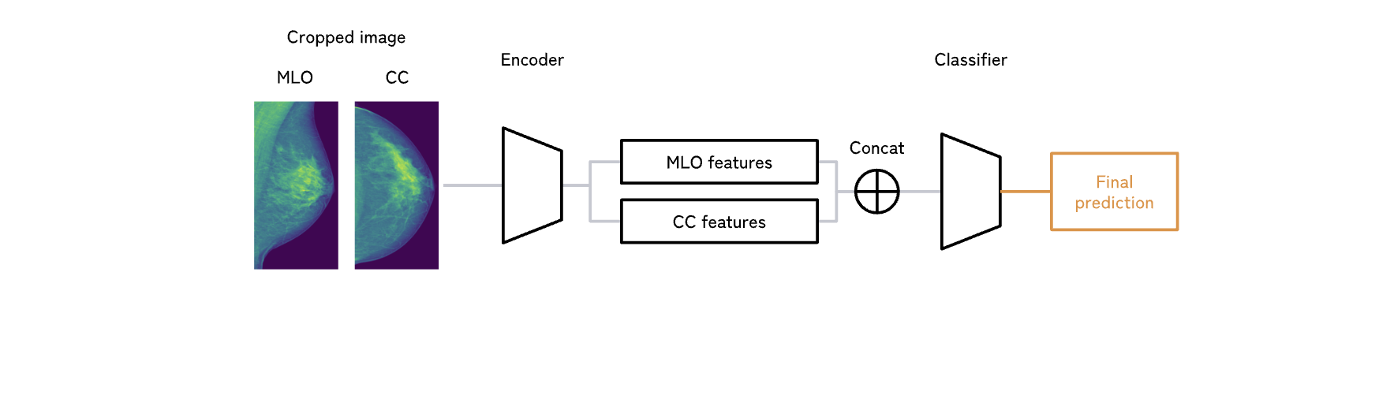
\includegraphics[scale = 0.6]{Figures/Award-winning Architecture 1.png}
   \caption{Basic Structure of the U-Net}
\end{figure}

\begin{figure}[htp]
    \centering
    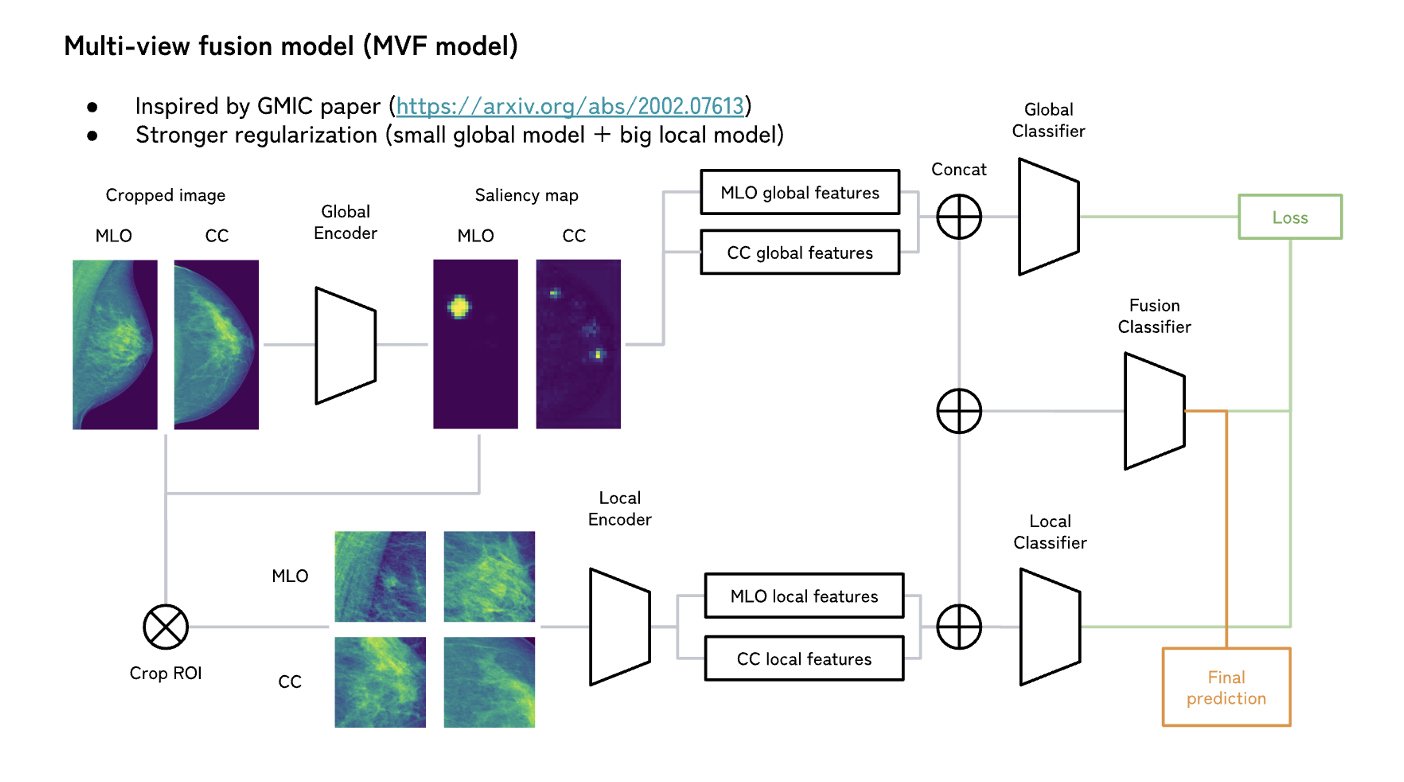
\includegraphics[scale = 0.6]{Figures/Award-winning Architecture 2.png}
   \caption{Basic Structure of the U-Net}
\end{figure}
\subsubsection{Efficient Net}
Efficient Net\cite{tan2019efficientnet} mainly introduces a new scaling method that balances network depth, width, and resolution to achieve better performance. The compound scaling method proposed in this paper is based on the observation that simply increasing the width, depth, or resolution of a ConvNet can lead to diminishing returns in terms of accuracy and efficiency. Instead, the authors propose a more principled approach that balances all three dimensions using a single compound coefficient $\phi$. 

The method involves scaling the depth, width, and resolution of the network according to the following equations:

\begin{equation}
d = \alpha^\phi, \quad w = \beta^\phi, \quad r = \gamma^\phi
\end{equation}

where $d$, $w$, and $r$ represent the depth, width, and resolution of the network respectively. The constants $\alpha$, $\beta$, and $\gamma$ are determined by a small grid search and subject to the constraint that $\alpha \cdot \beta^2 \cdot \gamma^2 \approx 2$. 

The authors show that this compound scaling method outperforms other single-dimension scaling methods on image classification tasks such as ImageNet. They also demonstrate that this approach can be used to efficiently scale up existing ConvNets without sacrificing accuracy. 

Overall, this paper provides a novel methodology for scaling ConvNets that achieves better accuracy and efficiency by balancing all dimensions of network width, depth, and resolution in a principled way using a single compound coefficient. Since this the model is commonly implemented in various competitions in Kaggle, we also adopt it as the baseline model.

\subsubsection{Vision-Transformer-Based Model}
\textbf{Architecture of Vision Transformer}

Vision transformers\cite{dosovitskiy2020image} are based on the transformer model originally used in natural language processing (NLP), which takes one-dimensional sequences of word tokens as input. However, since images are two-dimensional, vision transformers partition them into smaller two-dimensional patches, which are then treated as word tokens in the transformer model. The input image, with height $H$, width $W$, and $C$ channels, is divided into $N=\frac{H W}{P^2}$ patches of size $P \times P$ to align with the input structure used in NLP \cite{ayana2022buvitnet}. Prior to feeding the patches to the transformer encoder, they undergo flattening, sequence embedding, learnable embedding, and patch embedding in the order shown below:
\begin{itemize}
\item Flattening each patch into a vector $X_{np}$, where $n = 1, \ldots, N$, with a length of $P^2 \times C$ was performed.
\item The flattened patches were then mapped to $D$ dimensions using a trainable linear projection $E$, producing a series of embedded image patches.
\item Adding to the input sequence, the sequence of embedded image patches was prefixed with a learnable class embedding $X_{class}$ that corresponded to the classification outcome $Y$.
\item Positional information was incorporated into the input by adding one-dimensional positional embeddings $E_{pos}$, which were also learned during training, to the patch embeddings.
\end{itemize}

The embedding vectors that are obtained from the operations mentioned above are expressed by $z_{0}$:
\begin{equation}
z_o=\left[X_{\text {class }} ; X_p^1 E ; \ldots ; X_p^N E\right]+E_{p o s}
\end{equation}


 The embedding vectors $z_o$ are input to the transformer-encoder network, which is a stack of $L$ identical layers, to conduct the classification task.At the $L$-th layer of the encoder output, the classification head is fed with the value of $X_{class}$. In the pretraining stage, a multilayer perceptron (MLP) with a single hidden layer implementing the GELU nonlinearity is utilized as the classification head. In the fine-tuning stage, a single linear layer is utilized as the classification head.

 The vision transformer utilizes the encoder components of the original NLP transformer architecture. The input consists of a sequence of embedded image patches of size 16 x 16, along with positional data and a learnable class embedding. A patch size of 16 x 16 was chosen to strike a balance between performance and computational cost. The learnable class embedding is fed to a classification head connected to the output of the encoder, which produces a classification output based on its state. Figure \ref{fig.vit} illustrates the model architecture based on the vision transformer. In this work, the original vision transformer model pre-trained on the ImageNet dataset was modified by replacing its last layer with a flattening layer followed by batch normalization and an output dense layer.

\begin{figure*}[h!]
\begin{flushleft}
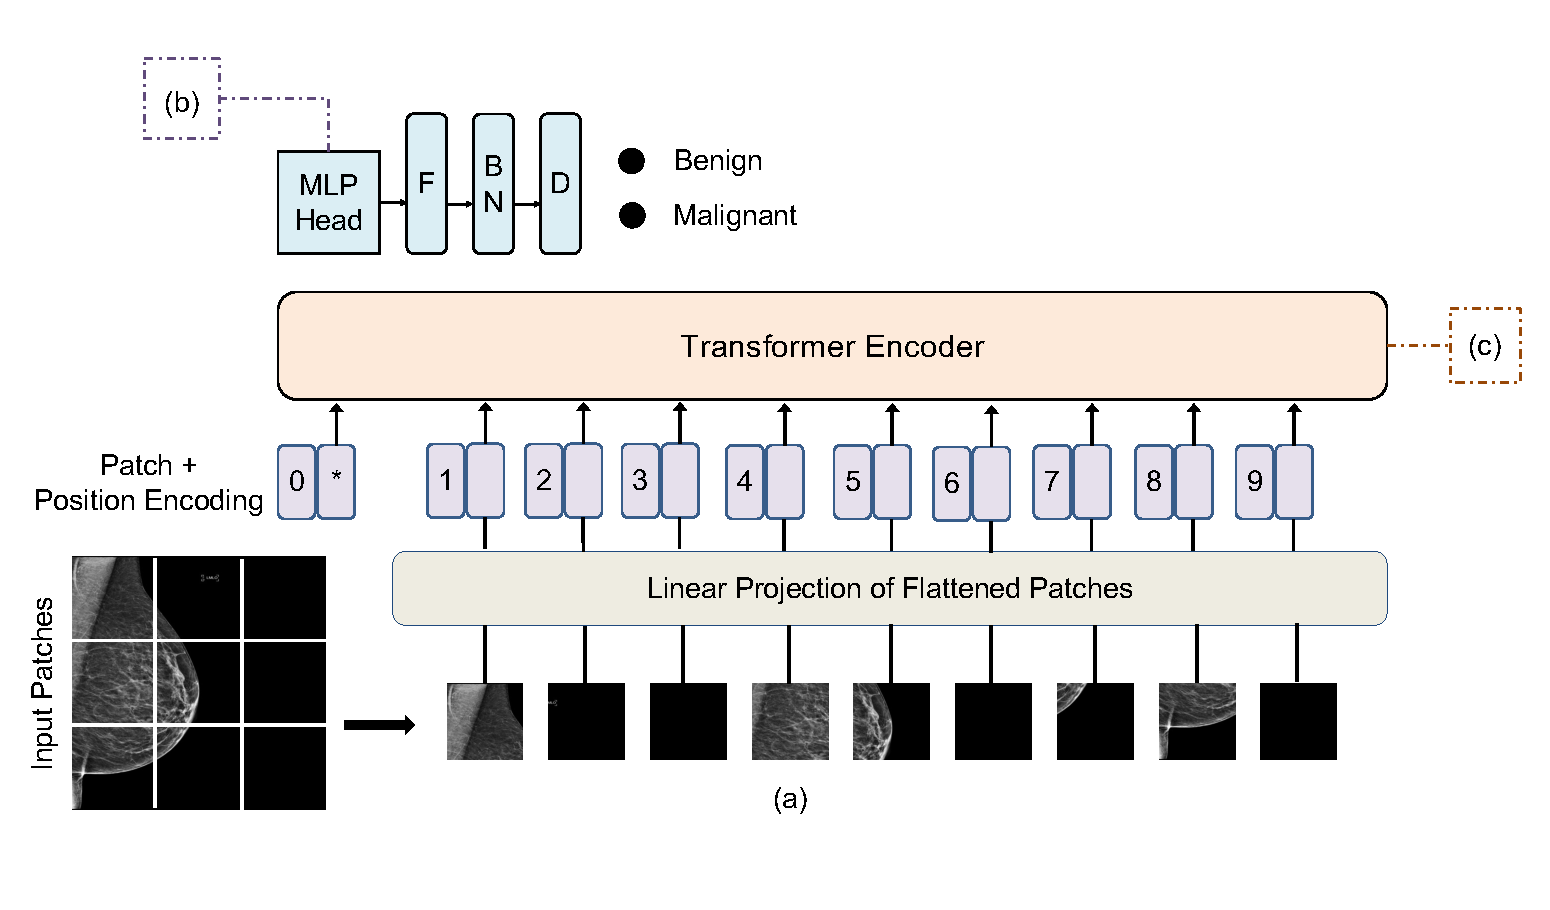
\includegraphics[width=\textwidth]{Figures/Vit_Archi_resize.pdf}
\caption{(a) Architecture of Vision Transformer applied to mammography breast cancer detection}
\label{fig.vit}
\end{flushleft}
\end{figure*}
\subsubsection{Transfer Learning}
Transfer learning was used to train vision transformer models on the mammography dataset using pre-trained examples from the vast ImageNet natural image dataset. The goal was to categorize breast mammograms into two classes—those from benign and malignant tissues—using the vision transformer's expertise from the substantial natural image collection. To do this, we removed the pre-trained prediction head and substituted a D $\times$ K feedforward layer, where K = 2 represents the total number of classes in the downstream direction. Our goal in this application of transfer learning was to improve our ability to learn the target function $f_t(\cdot)$ in the target domain $D_t$ by drawing on our prior understanding of the source domain $D_s$ and the learning task $T_s$. There are $m$ training examples $\left\{\left(x^1, y^1\right), \ldots,\left(x^i, y^i\right), \ldots,\left(x^m, y^m\right)\right\}$ in the ImageNet dataset, with $x^i$ denoting the ith input and $y^i$ the ith label. By then minimizing the objective function in equation\ref{eq.transfer}, where $\left\langle y^{i j} \mid x^{i j}, W_0, W_1, b\right\rangle$ is the Softmax output probability function, and $b$ is the bias, $W_1$ was generated using the weights of the ImageNet pre-trained vision transformer model $W_0$.

\begin{equation}
J\left(\left\langle W_1, b \mid W_0\right\rangle\right)=\frac{-1}{m n} \sum_{i=1}^m \sum_{j=1}^m y^{i j} \log \left(P\left\langle y^{i j} \mid x^{i j}, W_0, W_1, b\right\rangle\right)
\label{eq.transfer}
\end{equation}

\section{Results}
\subsection{Experimental setup}
In this task, what we predict is the likelihood of each breast of each patient that getting cancered.We compared the performance of the Vision Transformer pretrained on ImageNet\cite{deng2009imagenet} with the Efficient Net on the same dataset: RSNA screening mammography breast cancer detection dataset. The training hyperparameters and model implenmentation details can see Table.\ref{table:training_hyperparameters}. 
\begin{table}[h!]
\centering
\begin{tabular}{ |c|c| }
\hline
Hyperparameter & Value \\
\hline
Learning rate & $2\times10^{-4}$ \\
Weight decay & $1\times10^{-5}$ \\
Batch size & 64 \\
Epoch number & 20 \\
Loss  &Binary cross-entropy with logits loss \\
Optimizer & Adam\\
Training and validating ratio & 4:1\\
\hline
\end{tabular}
\caption{Training hyperparameters of the implemented model.  }
\label{table:training_hyperparameters}
\end{table}

\subsection{Evaluation Metric}
In this task, we adopt the probabilistic F1 score \cite{yacouby2020probabilistic} for performance evaluation. Probabilistic F1 score is an extension of the traditional F1 score that takes into account the uncertainty of a model's predictions. It is a metric used to evaluate classification models in natural language processing. The Probabilistic F1 score considers both precision and recall, as well as the confidence level of the model's predictions. This allows for a more thorough evaluation of the model's performance, especially in cases where there are razor-thin margins and low-resource test sets.
The mathematical formulation of probabilistic F1 score is shown below.
\begin{equation}
p T P_{C_j}=M\left(\mathbf{x}_{\mathbf{i}}, C_j\right) * I_{C_j=y_i}
\end{equation}
\begin{equation}
p F P_{C_j}=M\left(\mathbf{x}_{\mathbf{i}}, C_j\right) * I_{C_j \neq y_i}
\end{equation}
\begin{equation}
\begin{gathered}
p \text { Precision }=\frac{p T P}{p T P+p F P} \\
p \text { Recall }=\frac{p T P}{p T P+p F N}
\end{gathered}
\end{equation}

Here $\mathbf{x}_{\mathbf{i}}$ denotes the ith sample, $C_j$ denotes the jth possible class, $y_i$ denotes the ith label. pTP, pFP, pPrecision, pRecall represents the probabilistic true positive,probabilistic false positive,probabilistic precision, probabilistic recall. 
\begin{equation}
pF_1 =\frac{2p Precision*pRecall}{p Precision+p Recall}
\end{equation}

\subsection{Experimental Results}
The experiment results are shown in Table\ref{table:result}.Five-fold cross-validation was used to compare the model performances. From the table, we can see that the vision-transformer-based transfer-learning approach provided the highest quantitative and statistical measures for predicting the likelihood of breast mammograms as being from benign or malignant tissues. This proves the effectiveness and quality of the vision-transformer-based transfer-learning approach for detecting breast cancer from mammograms. The possible reason is that vision transformer has the ability to capture global information from the early layers and the deep self-attention mechanism that enables features in each patch to be carefully analyzed for decision making.

\renewcommand{\heavyrulewidth}{1.1pt}
\begin{table}[h!]
\centering
\begin{tabular}{ ccccc }
\toprule
Model & pF1 Score &pPrecision &pRecall &pAUROC\\
\midrule
EfficientNetV2\cite{tan2021efficientnetv2} & 0.45 &0.45 &0.46 &0.44 \\
Vit-base &  0.52 & 0.53 &0.52 &0.52\\

\bottomrule
\end{tabular}

\caption{Testing Result on RSNA Screening Mammography Breast Cancer Detection Dataset}
\label{table:result}
\end{table}


\section{Future Work \& Conclusion}


\subsection{Limitations}
\textbf{Lack of in-depth Feature Analysis}\\
For each patient, there is four mammography images(Left/Right with two kinds of image-forming condition), so the features may have some inner correlations. However, in the project, we omit this information and does not come up with a method to extract more useful information from the inner correlation between these four images.

\textbf{Multi-View Fusion Model}\\
In the recent year, multi-view fusion model is really a hot topic. For example, in the Mei et al.\cite{mei2018unsupervised}'s work, they proposed the pyramid image fusion method to train the model.  The pyramid structure allows for the extraction of features at different scales, which are then synthesized using a multimodal strategy to improve the robustness and accuracy of the method. The idea of cropping the image to different scales to catch both the global features and the local features may also be suitable for this project.


\subsection{Further Study}


\section{Author contributions}
Chenglin Zhang: \\
Lihui Chen: \\
Yijia Xue: Implementing the Vision Transformer. Report Writing: includes the section related to Efficient Net/ Vision Transformer/Transfer Learning/Results/Model Limitations\\
\section{Acknowledgement}
We thank Prof. Dongmian Zou for the generous and insightful guidance in this session's Deep Learning course, that it will empower our future learning greatly.

\clearpage
    
\clearpage

\bibliographystyle{unsrt}  
\bibliography{references}  


\end{document}
